\documentclass[a4paper]{article}

\usepackage[T1]{fontenc}
\usepackage[italian]{babel}
\usepackage[latin1]{inputenc}
\usepackage{graphicx}
\usepackage{float}
\usepackage[margin=2.5cm]{geometry}
\usepackage{multirow}
\usepackage{multicol}
\usepackage{url}
\author{Alberto Bordin, Giulio Cappelli}
\title{Interferometro di Michelson}
\date{6-7 novembre 2017}
\newcommand{\minitab}[2][l]{\begin{tabular}#1 #2\end{tabular}}


\begin{document}
	\maketitle
	
	\begin{abstract}
		 Misura della lunghezza d'onda di tre diversi laser.
		 
		 Misura di spostamenti micrometrici: isteresi di un piezoelettrico.
		 
		 Misura dell'indice di rifrazione dell'aria.
	\end{abstract}

\begin{multicols}{2}

\section{Teoria}
\begin{center}
	\begin{minipage}[c]{.50\textwidth}
		\centering
		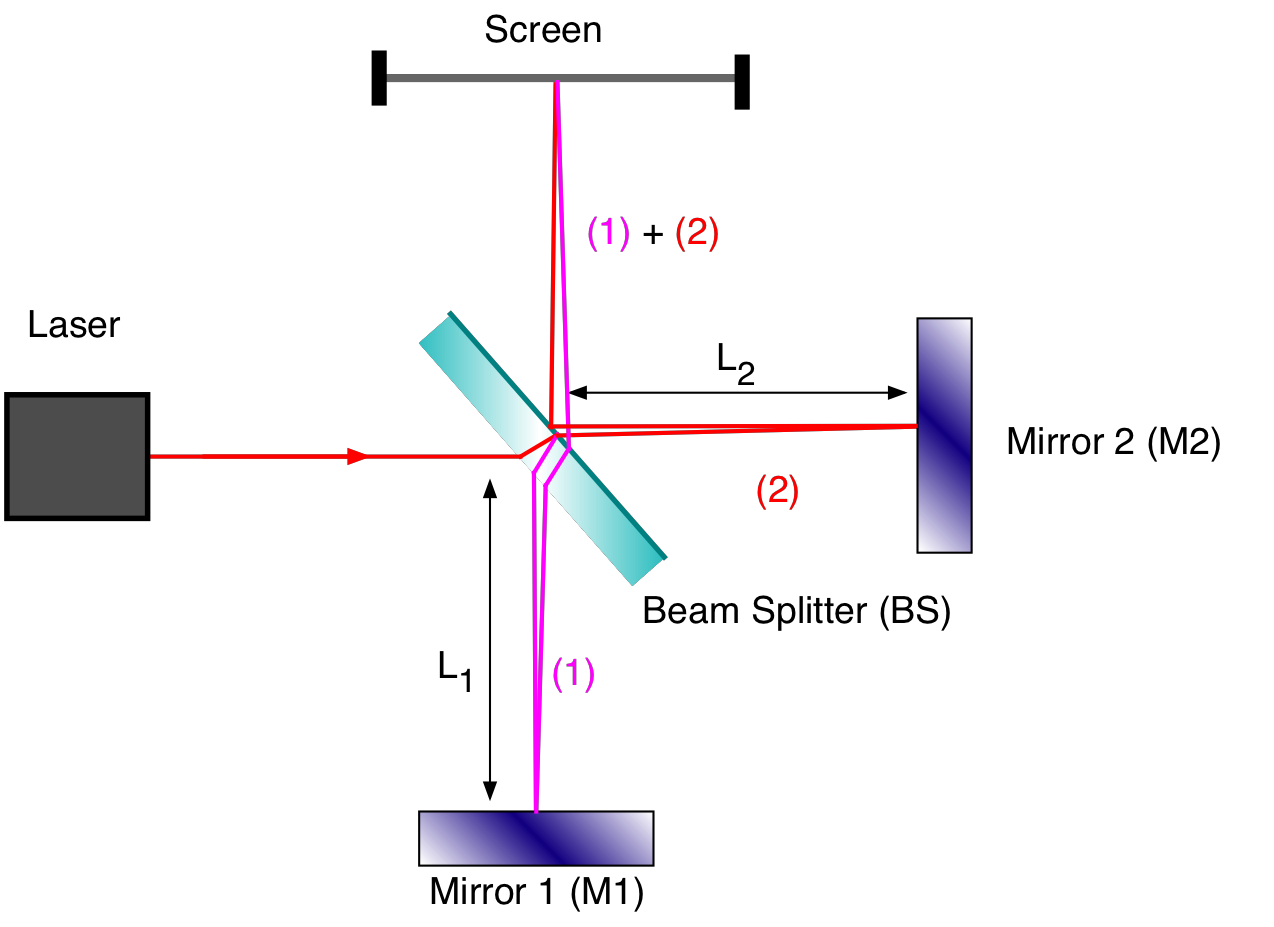
\includegraphics[width=1\textwidth]{teoria_michelson.png}
	\end{minipage}
\end{center}
In un interferometro di Michelson come quello in figura la condizione per avere interferenza costruttiva~� 
\begin{equation}
2(L_1 -L_2)n = m \lambda\ 
\label{eq:interferenza}
\end{equation}
dove $n$ � l'indice di rifrazione dell'aria e $m$ � il numero di frange. Nel nostro apparato variamo $L_2$ e contiamo la corrispondente variazione di $m$.


\section{Apparato sperimetale}

	Abbiamo a disposizione 
	\begin{itemize}
		\item Tre laser di diversa lunghezza d'onda: 633 nm (laser HeNe), 650 nm, 532 nm.
		\item Un interferometro di Michelson a divisione di ampiezza.
		\item Un rilevatore al silicio (fotodiodo) per misurare l'intensit� luminosa.
		\item Un piezoelettrico.
		\item Un multimetro digitale.
		\item Una camera a vuoto lunga 5 cm $\pm$ 50 $\mu$m.
		\item Una pompa a vuoto.
		\item Un motorino passo passo che mette in rotazione una vite micrometrica.
		\begin{figure}[H]
			\centering
			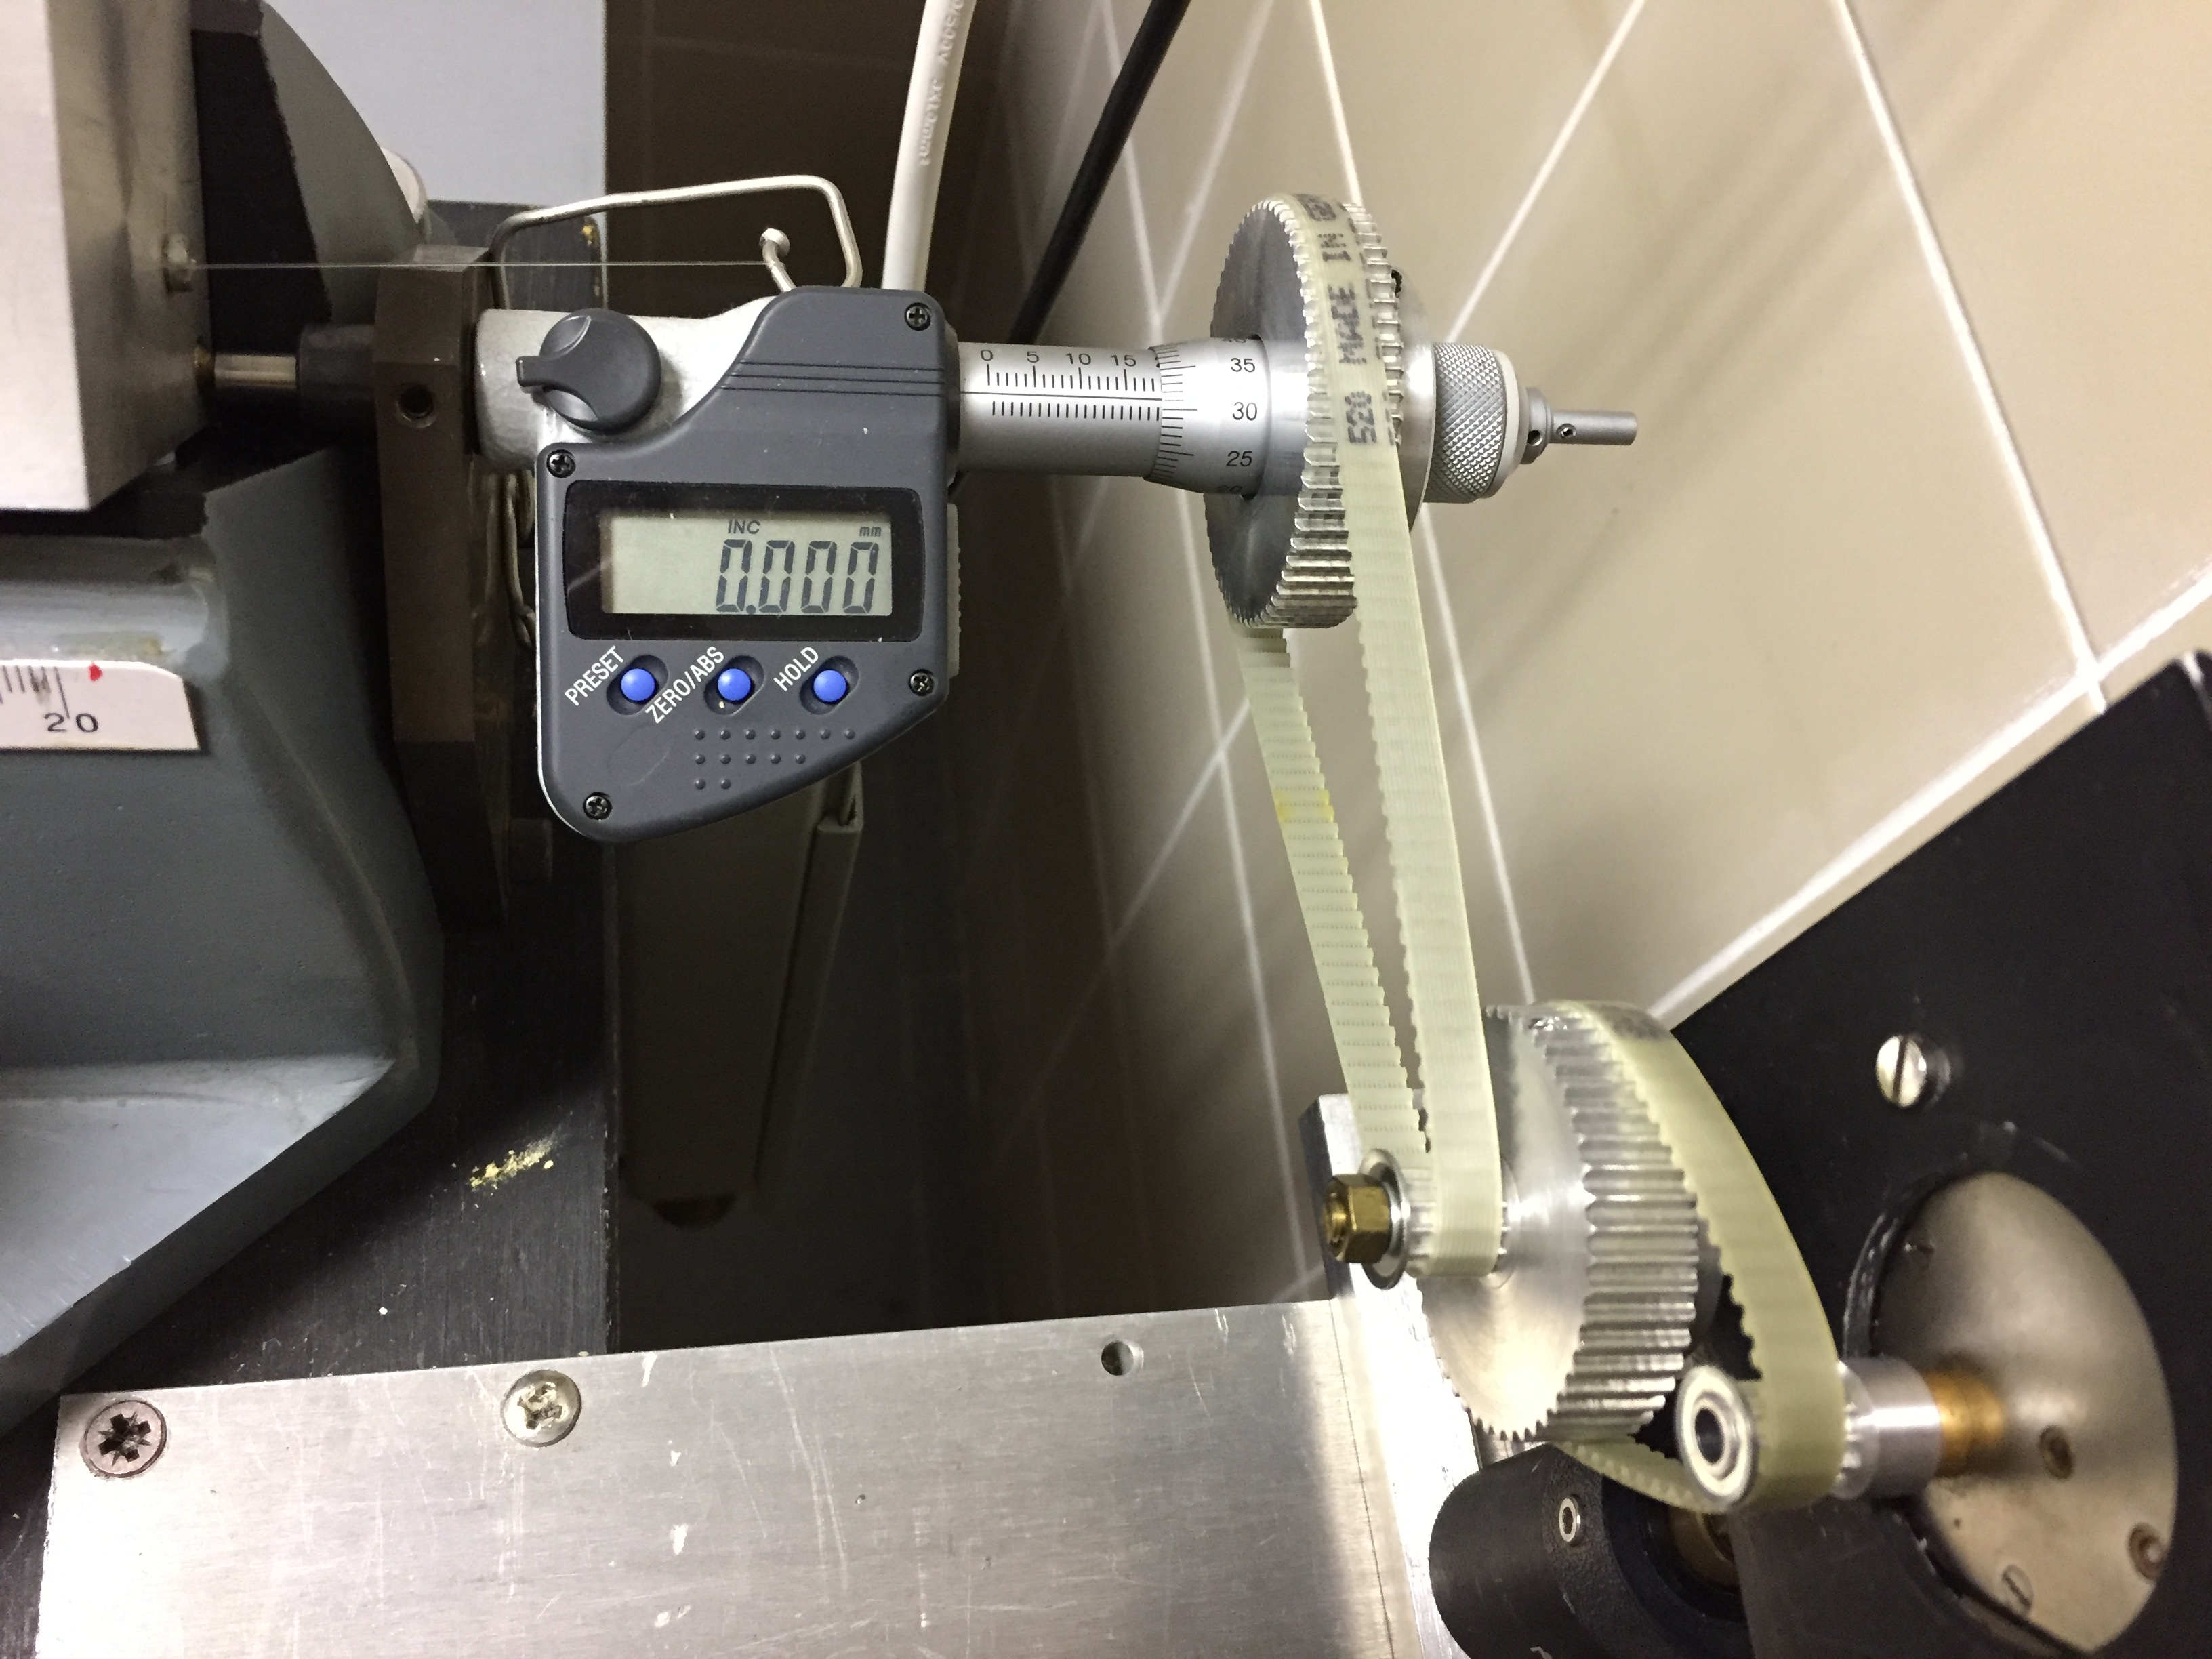
\includegraphics[width=0.4\textwidth]{vite_micrometrica.JPG}
		\end{figure}


	\end{itemize}
Il principio di funzionamento � l'interferenza a divisione di ampiezza. Per avere interferenza al finito usiamo una lente, che trasforma onde piane in onde sferiche. Le frange di interferenza vengono rivelate tramite un fotodiodo il cui segnale viene letto al PC tramite un VI labVIEW, che salva anche i dati.

\section{Misura della lunghezza \\d'onda}
Per misurare la lunghezza d'onda del laser contiamo le frange di interferenza al variare della differenza di cammino ottico. 

\subsection{Presa dati}
Per prima cosa allineiamo il fascio laser in modo da vedere delle frange di interferenza definite sul rilevatore al silicio. 
Poi variamo la differenza di cammino ottico utilizzando un motorino passo passo collegato ad una vite micrometrica che muove lentamente uno degli specchi (M2). Il motorino si muove ad una velocit� di 125 step/s che corrispondono ad un avanzamento della vite di circa 0.4 $\mu$m/s; vediamo passare circa una frangia al secondo.
Al PC vediamo l'evoluzione delle frange di interferenza grazie ad un VI labVIEW, come in Figura \ref{fig:esempio_acquisizione_frange}.

\end{multicols}

\begin{figure}[H]
	\centering
	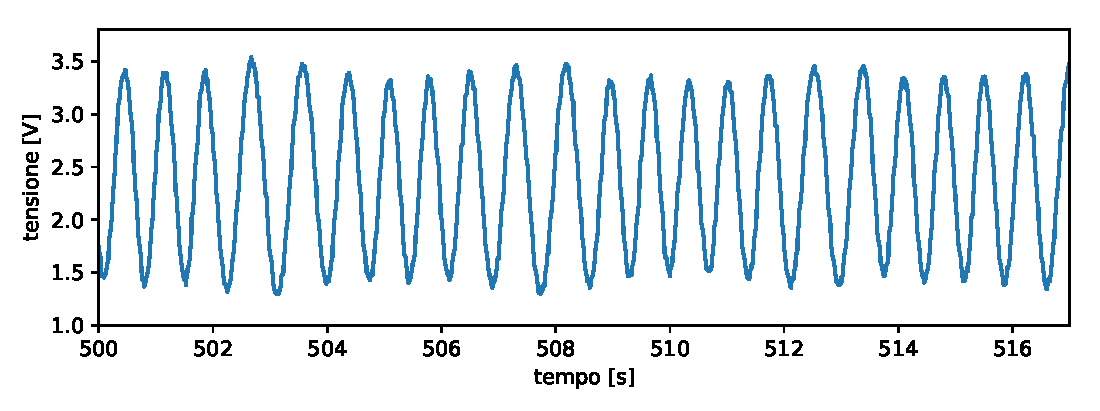
\includegraphics[width=1\textwidth]{esempio_acquisizione_frange.pdf}
	\caption{Esempio di acquisizione delle frange di interferenza.}
	\label{fig:esempio_acquisizione_frange}
\end{figure}

\begin{multicols}{2}

Al termine dell'acquisizione il VI fornisce il numero $m$ di picchi e il display digitale della vite micrometrica fornisce la distanza percorsa dallo specchio M2 che usiamo per calcolare la lunghezza d'onda tramite l'equazione \ref{eq:interferenza}.

\subsubsection{Accorgimenti sperimentali}
\begin{itemize}
	\item Per avere un buon segnale allineiamo il fascio laser prima di inserire la lente divergente e dopo averla inserita perfezioniamo la regolazione degli specchi in modo che le frange di interferenza siano larghe in corrispondenza del rivelatore (vedi Figura \ref{fig:frange}).
	\item Dato che il rilevatore al silicio � sensibile ad un ampio spettro verifichiamo che l'effetto della luce ambientale non disturbi il segnale.
	\item Stimiamo che l'errore sul conteggio dei picchi derivi soprattutto dai transienti di accensione e spegnimento del motorino e del VI, quindi li facciamo partire e fermare in contemporanea. Avviamo noi la partenza simultanea del motorino e della acquisizione, mentre per la fine impostiamo un fissato numero di step del motorino passo passo (modalit� F2) e una durata corrispondente nel programma di acquisizione (tempo $t$ in Tabella \ref{tab:lambda}).
	
	Inoltre scegliamo di impostare il massimo numero di step consentiti dal motorino (99999), questo minimizza l'errore sui transienti di accensione e spegnimento.\footnote{A parit� di tempo speso in laboratorio conviene fare una simulazione lunga piuttosto che fare la media di tante brevi. Se facciamo k acquisizioni tali che la durata complessiva sia N secondi l'errore sulla media va come $\frac{1}{\sqrt{k}}$ per l'errore su una acquisizione, che va come $\frac{1}{\frac{N}{k}}$. Quindi l'errore sulla media � proporzionale a $\frac{\sqrt{k}}{N}$. Conviene $k=1$.}
	\item Per evitare eventuali sistematiche dovute al verso di rotazione della vite alterniamo la direzione di moto del motorino (A e B in Tabella~\ref{tab:lambda}).
\end{itemize}

\begin{figure}[H]
	\centering
	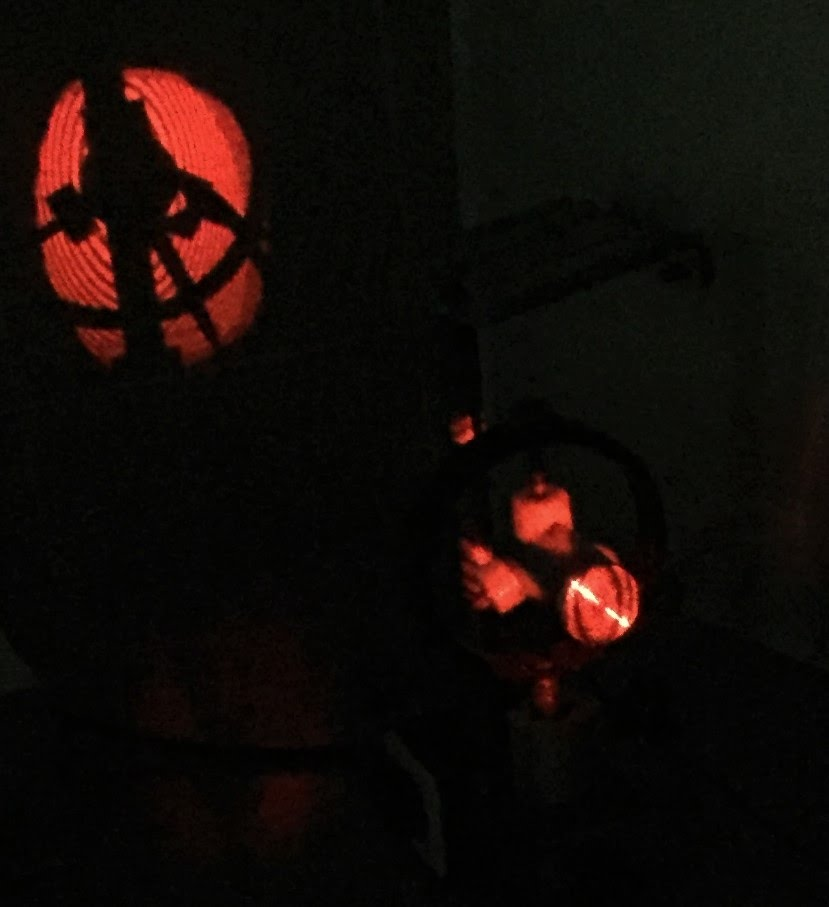
\includegraphics[width=0.3\textwidth]{frange.jpg}
	\caption{Frange di interferenza sul rilevatore.}
	\label{fig:frange}
\end{figure}

\subsection{Analisi dei dati}
Di seguito riportiamo le misure con i relativi errori. L'errore sulla distanza � la sensibilit� della vite, mentre quello sul numero di conteggi � stimato dalle differenze tra gli $m$ misurati.\footnote{Per le misure di $m$ di ciascun laser calcoliamo la deviazione standard, poi facciamo la media quadratica delle 3.}

\end{multicols}

\begin{table}[H]
	\centering
	\begin{tabular}{|c|ccccc|}
		\hline
		& $m(\Delta m)$ & $d(\Delta d)$ [$\mu$m] & $t$ [mm:ss] &$\lambda(\Delta\lambda)$ [nm] & direzione \\
		\hline
		\multirow{3}*{\minitab[c]{laser HeNe \\ (633 nm)}}
		& 1088(5) & 345(1) & 13:33 & 634(3) & A\\ 
		& 1094(5) &345(1) & 13:43 & 631(3) & B\\ 
		& 1092(5) &345(1) & 13:36 & 632(3) & A\\ 
		\hline
		\multirow{2}*{\minitab[c]{laser rosso \\ (650 nm)}}
		& 1065(5) &345(1) & 13:36 &  648(4) & A\\ 
		& 1054(5) &346(1) & 13:32 & 657(4) & B\\
		\hline
		\multirow{2}*{\minitab[c]{laser verde \\ (532 nm)}}
		& 1306(5) &347(1) & 13:32 & 531(3) & A\\
		& 1293(5) &347(1) & 13:32 & 537(3) & B\\
		\hline
	\end{tabular}
\caption{Dati grezzi e calcolo della lunghezza d'onda.}
	\label{tab:lambda}
\end{table}

\begin{multicols}{2}

\subsection{Conclusioni}
Per ogni laser abbiamo fatto la media dei valori di $\lambda$ misurati.
I risultati sono compatibili con quanto riportato nei datasheet. 

\begin{table}[H]
	\centering
	\begin{tabular}{|c|c|c|}
		\hline
		laser &$\lambda$ nominale [nm]& $\lambda(\Delta\lambda)$ misurata [nm]\\
		\hline
		HeNe & 632.8 & 632(2)\\
		rosso & 650 & 652(3)\\
		verde & 532 & 534(2)\\
		\hline
	\end{tabular}
\end{table}

\section{Isteresi del piezoelettrico}

In questa sezione diamo per nota $\lambda = 633$ nm e usiamo la formula $2dn = m\lambda$ per calcolare la differenza di cammino ottico $d$, ottenuta variando la tensione di alimentazione di un piezoelettrico. Eseguendo una spazzata da 0 a 100 V seguita da una da 100 a 0 V il piezoelettrico mostra un ciclo di isteresi, che andiamo ad analizzare.

\subsection{Presa dati}
Misuriamo l'alimentazione del piezoelettrico con un voltmetro collegato al PC. Il programma di acquisizione ci permette di salvare la tensione in funzione del tempo $V(t)$.
Simultaneamente avviamo il VI che conta le frange rilevate dal fotodiodo. Tramite uno script in python\footnote{Tutti i dati grezzi e gli script di analisi sono reperibili su https://github.com/albord95/relazioni-lab-ottica-quantistica/tree/master/Analizzatore\%20di\%20spettro/dati\%20e\%20script \\ Per eseguire gli script scaricare tutta la cartella dati-e-script. Serve python 3 con i pacchetti pylab, scipy, uncertainties, gvar e glob.\label{ftn:link}} leggiamo il file .txt salvato dal VI ed estraiamo il tempo $t$ di ogni massimo e minimo. Infine inseriamo tali tempi nella curva $V(t)$ ottenendo un grafico $d-V$ con 2 punti ogni frangia (vedi Figura \ref{fig:esempio_acquisizione_isteresi}).

\begin{figure}[H]
	\centering
	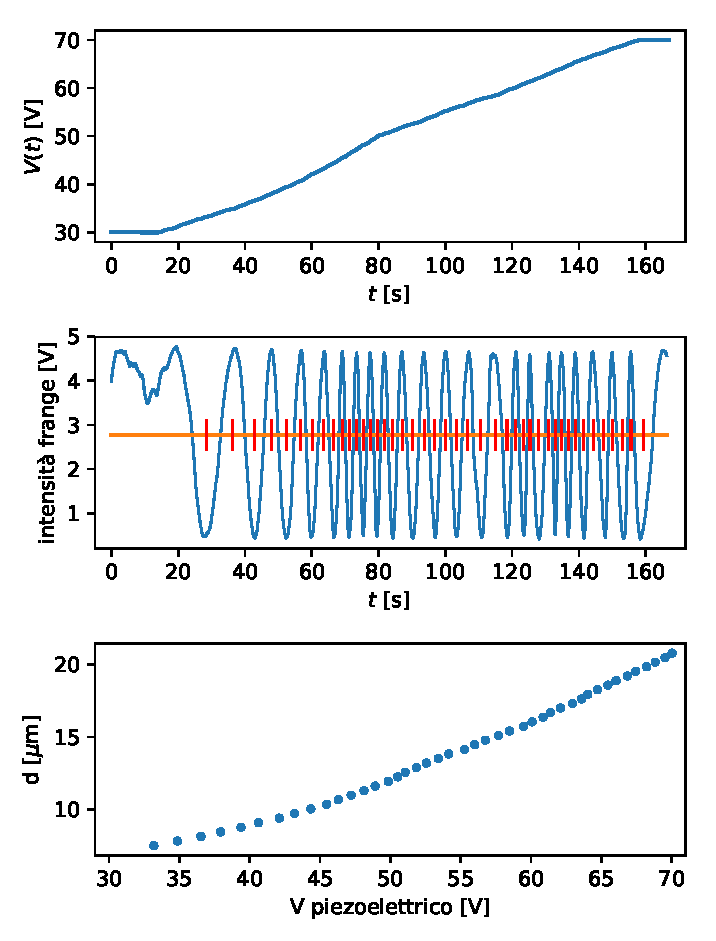
\includegraphics[width=0.5\textwidth]{esempio_acquisizione_isteresi.pdf}
	\caption{Esempio di acquisizione della curva del piezoelettrico.}
	\label{fig:esempio_acquisizione_isteresi}
\end{figure}

\subsection{Analisi dati}

\subsubsection{Alimentazione da 0 a 100 Volt}
In Figura \ref{fig:0-100} vediamo il ciclo di isteresi seguito dal piezoelettrico. Per valutarne la (non)linearit� abbiamo deciso di confrontare le pendenze della prima e della seconda met� di ogni rampa. Abbiamo eseguito un fit lineare: confrontando i coefficienti angolari notiamo non solo che sono statisticamente incompatibili, ma che sono diversi gi� alla prima cifra.
L'errore sull'alimentazione � dato dalla fluttuazione del valore letto al multimetro (0.2 V) mentre l'errore su $d$ � la distanza tra due frange.

\end{multicols}

\begin{figure}[H]
	\centering
	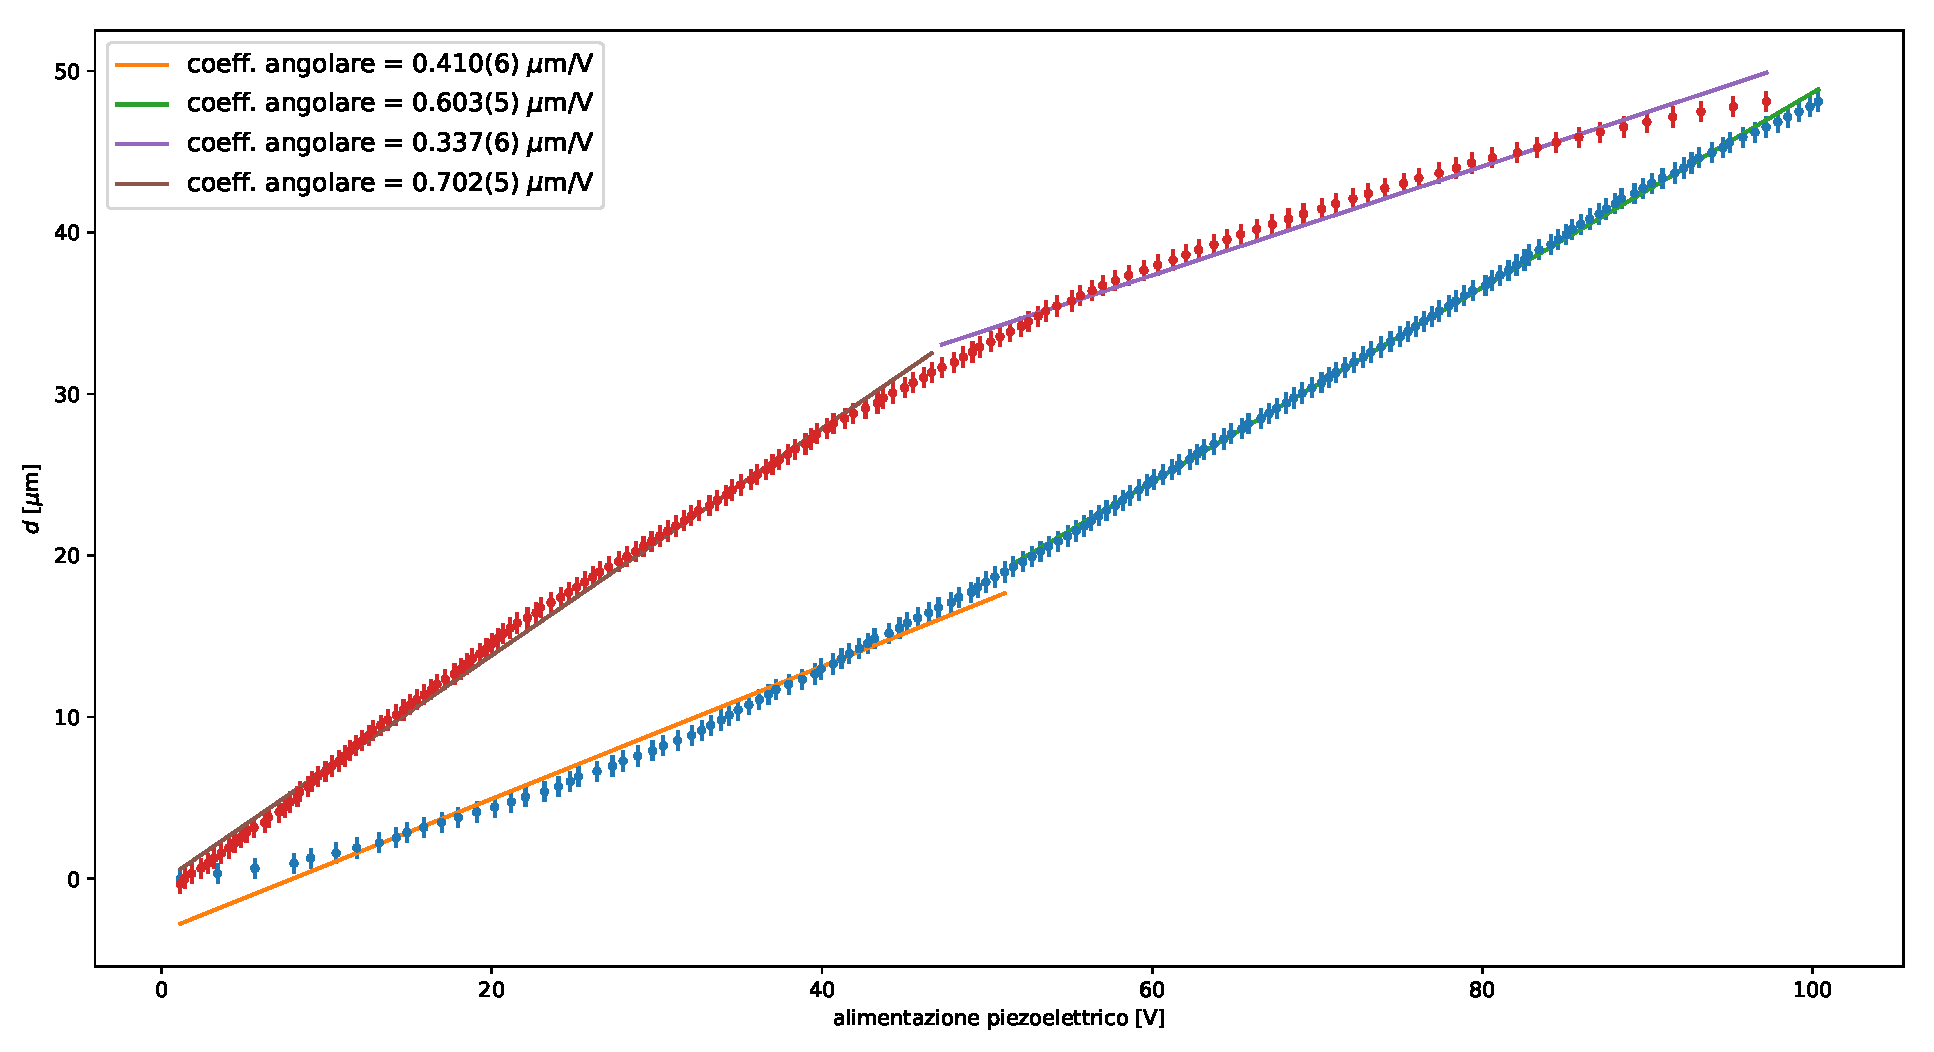
\includegraphics[width=1\textwidth]{isteresi_0-100.pdf}
	\caption{Isteresi del piezoelettrico: 0-100 V.}
	\label{fig:0-100}
\end{figure}

\begin{multicols}{2}

\subsubsection{Alimentazione da 30 a 70 Volt}
Ripetiamo la stessa analisi variando l'alimentazione del piezoelettrico da 30 a 70 V (vedi Figura \ref{fig:30-70-1}). Questo dovrebbe essere il regime lineare e in effetti l'isteresi � meno evidente, tuttavia i coefficienti angolari fittati restano incompatibili.

\end{multicols}

\begin{figure}[H]
	\centering
	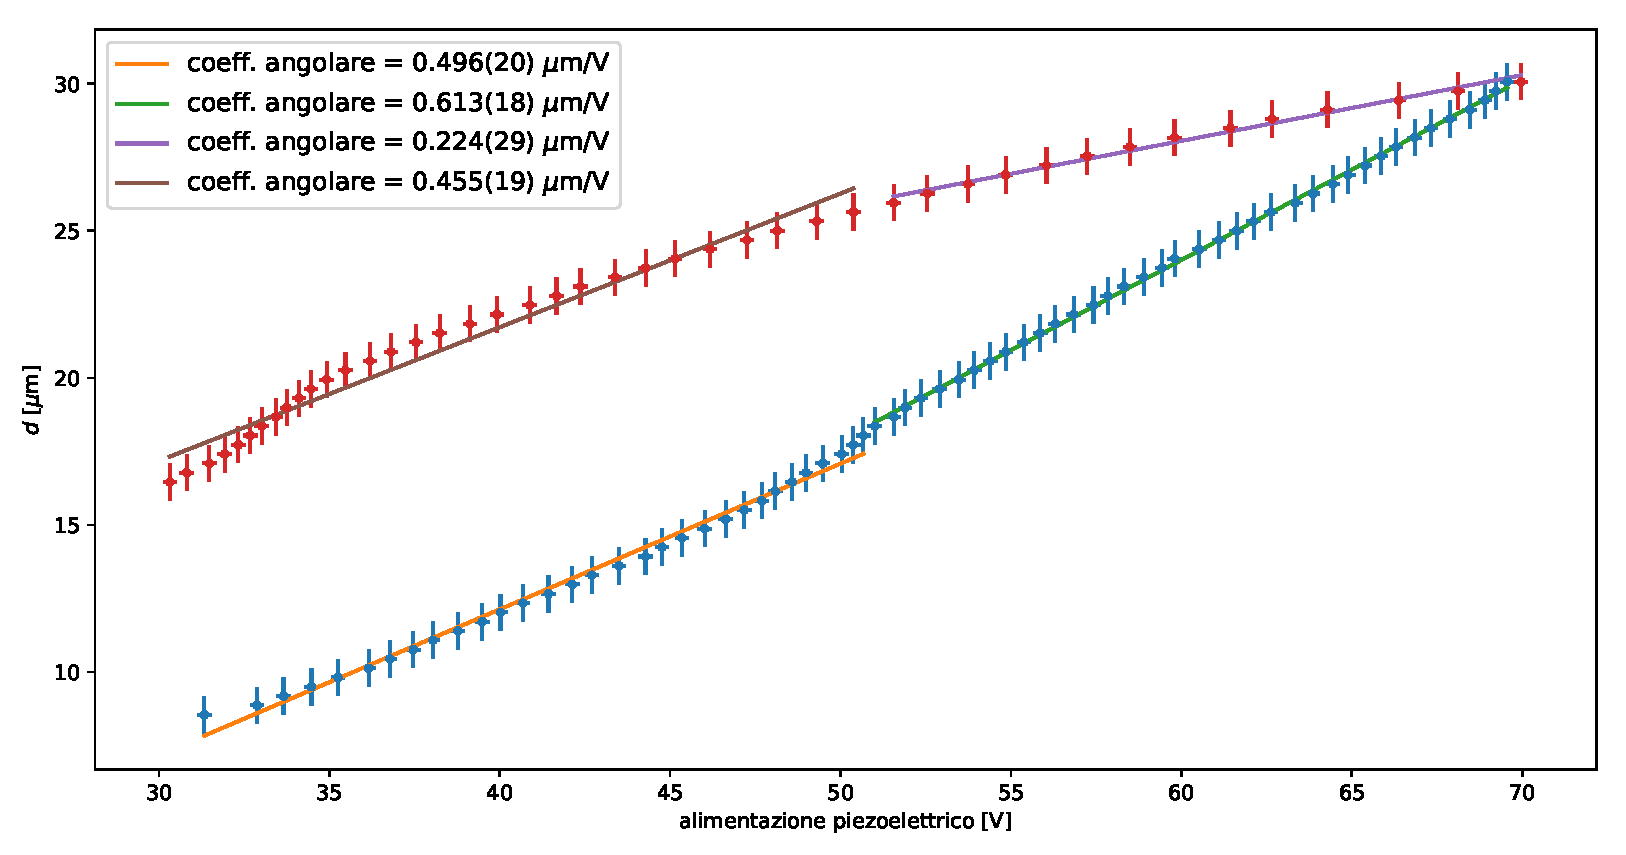
\includegraphics[width=1\textwidth]{isteresi_30-70-1.pdf}
	\caption{Isteresi del piezoelettrico: 30-70 V.}
	\label{fig:30-70-1}
\end{figure}

\begin{multicols}{2}

 In Figura \ref{fig:30-70-1} si nota anche che il ciclo non si chiude, ci� avviene perch� i 30 V dell'inizio della salita sono stati raggiunti salendo da 0 V, quindi il punto a 30 V risente dell'isteresi da 0 a 70 V. Abbiamo verificato che, finita la discesa da 70 a 30 V, risalendo, il ciclo si richiudesse a 70 V come si nota in Figura \ref{fig:30-70-2}. Iterando nuovamente salita e discesa i cicli resterebbero chiusi.
 
 \end{multicols}
 
 \begin{figure}[H]
 	\centering
 	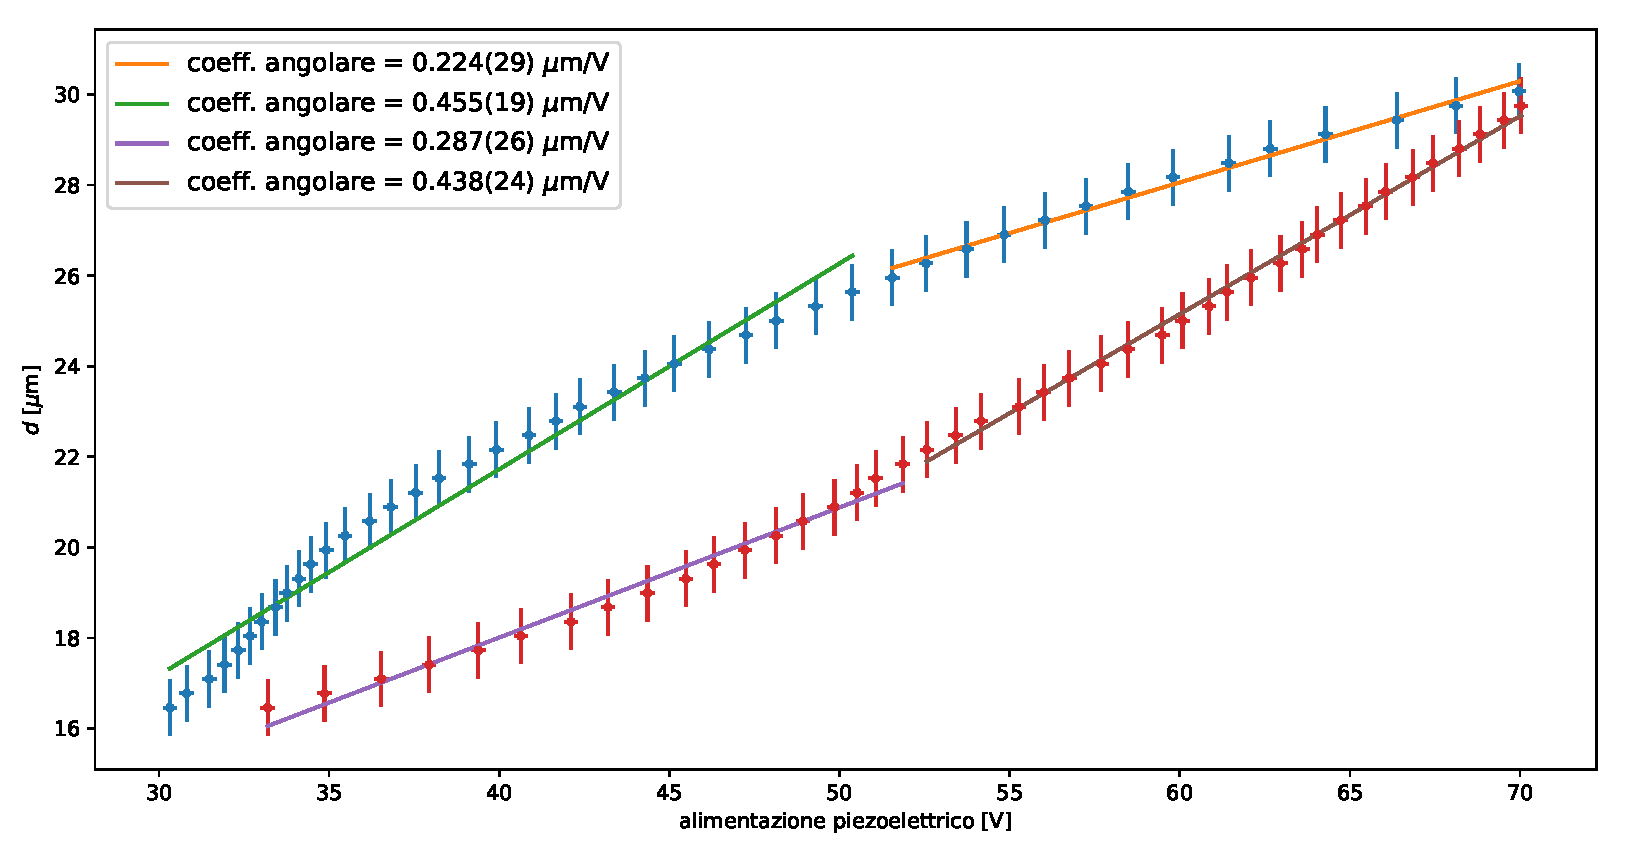
\includegraphics[width=1\textwidth]{isteresi_30-70-2.pdf}
 	\caption{Isteresi del piezoelettrico: 30-70 V.}
 	\label{fig:30-70-2}
 \end{figure}
 
 \begin{multicols}{2}

\subsection{Conclusioni}
Abbiamo osservato il ciclo di isteresi del piezoelettrico. Abbiamo constatato che tra 30 e 70~V la non-linearit� � ridotta, ma ancora visibile. 

\section{Indice di rifrazione dell'aria}

Utilizziamo adesso l'interferometro di Michelson per misurare l'indice di rifrazione di un mezzo in cui si propaga la luce laser nota la sua lunghezza d'onda e la distanza percorsa dal fascio nel mezzo. 

\subsection{Presa dati}
Per farlo inseriamo nel percorso del fascio laser, fra il beam splitter e lo specchio M1, la camera a vuoto mostrata in Figura \ref{fig:cv} e attraverso una pompa facciamo il vuoto al suo interno.\footnote{Per assicurarci di ottenere la migliore condizione di vuoto abbiamo lasciato accesa la pompa finch� vedevamo le frange scorrere sul rilevatore, per un tempo medio di circa 5 minuti.}

 \begin{figure}[H]
 	\centering
 	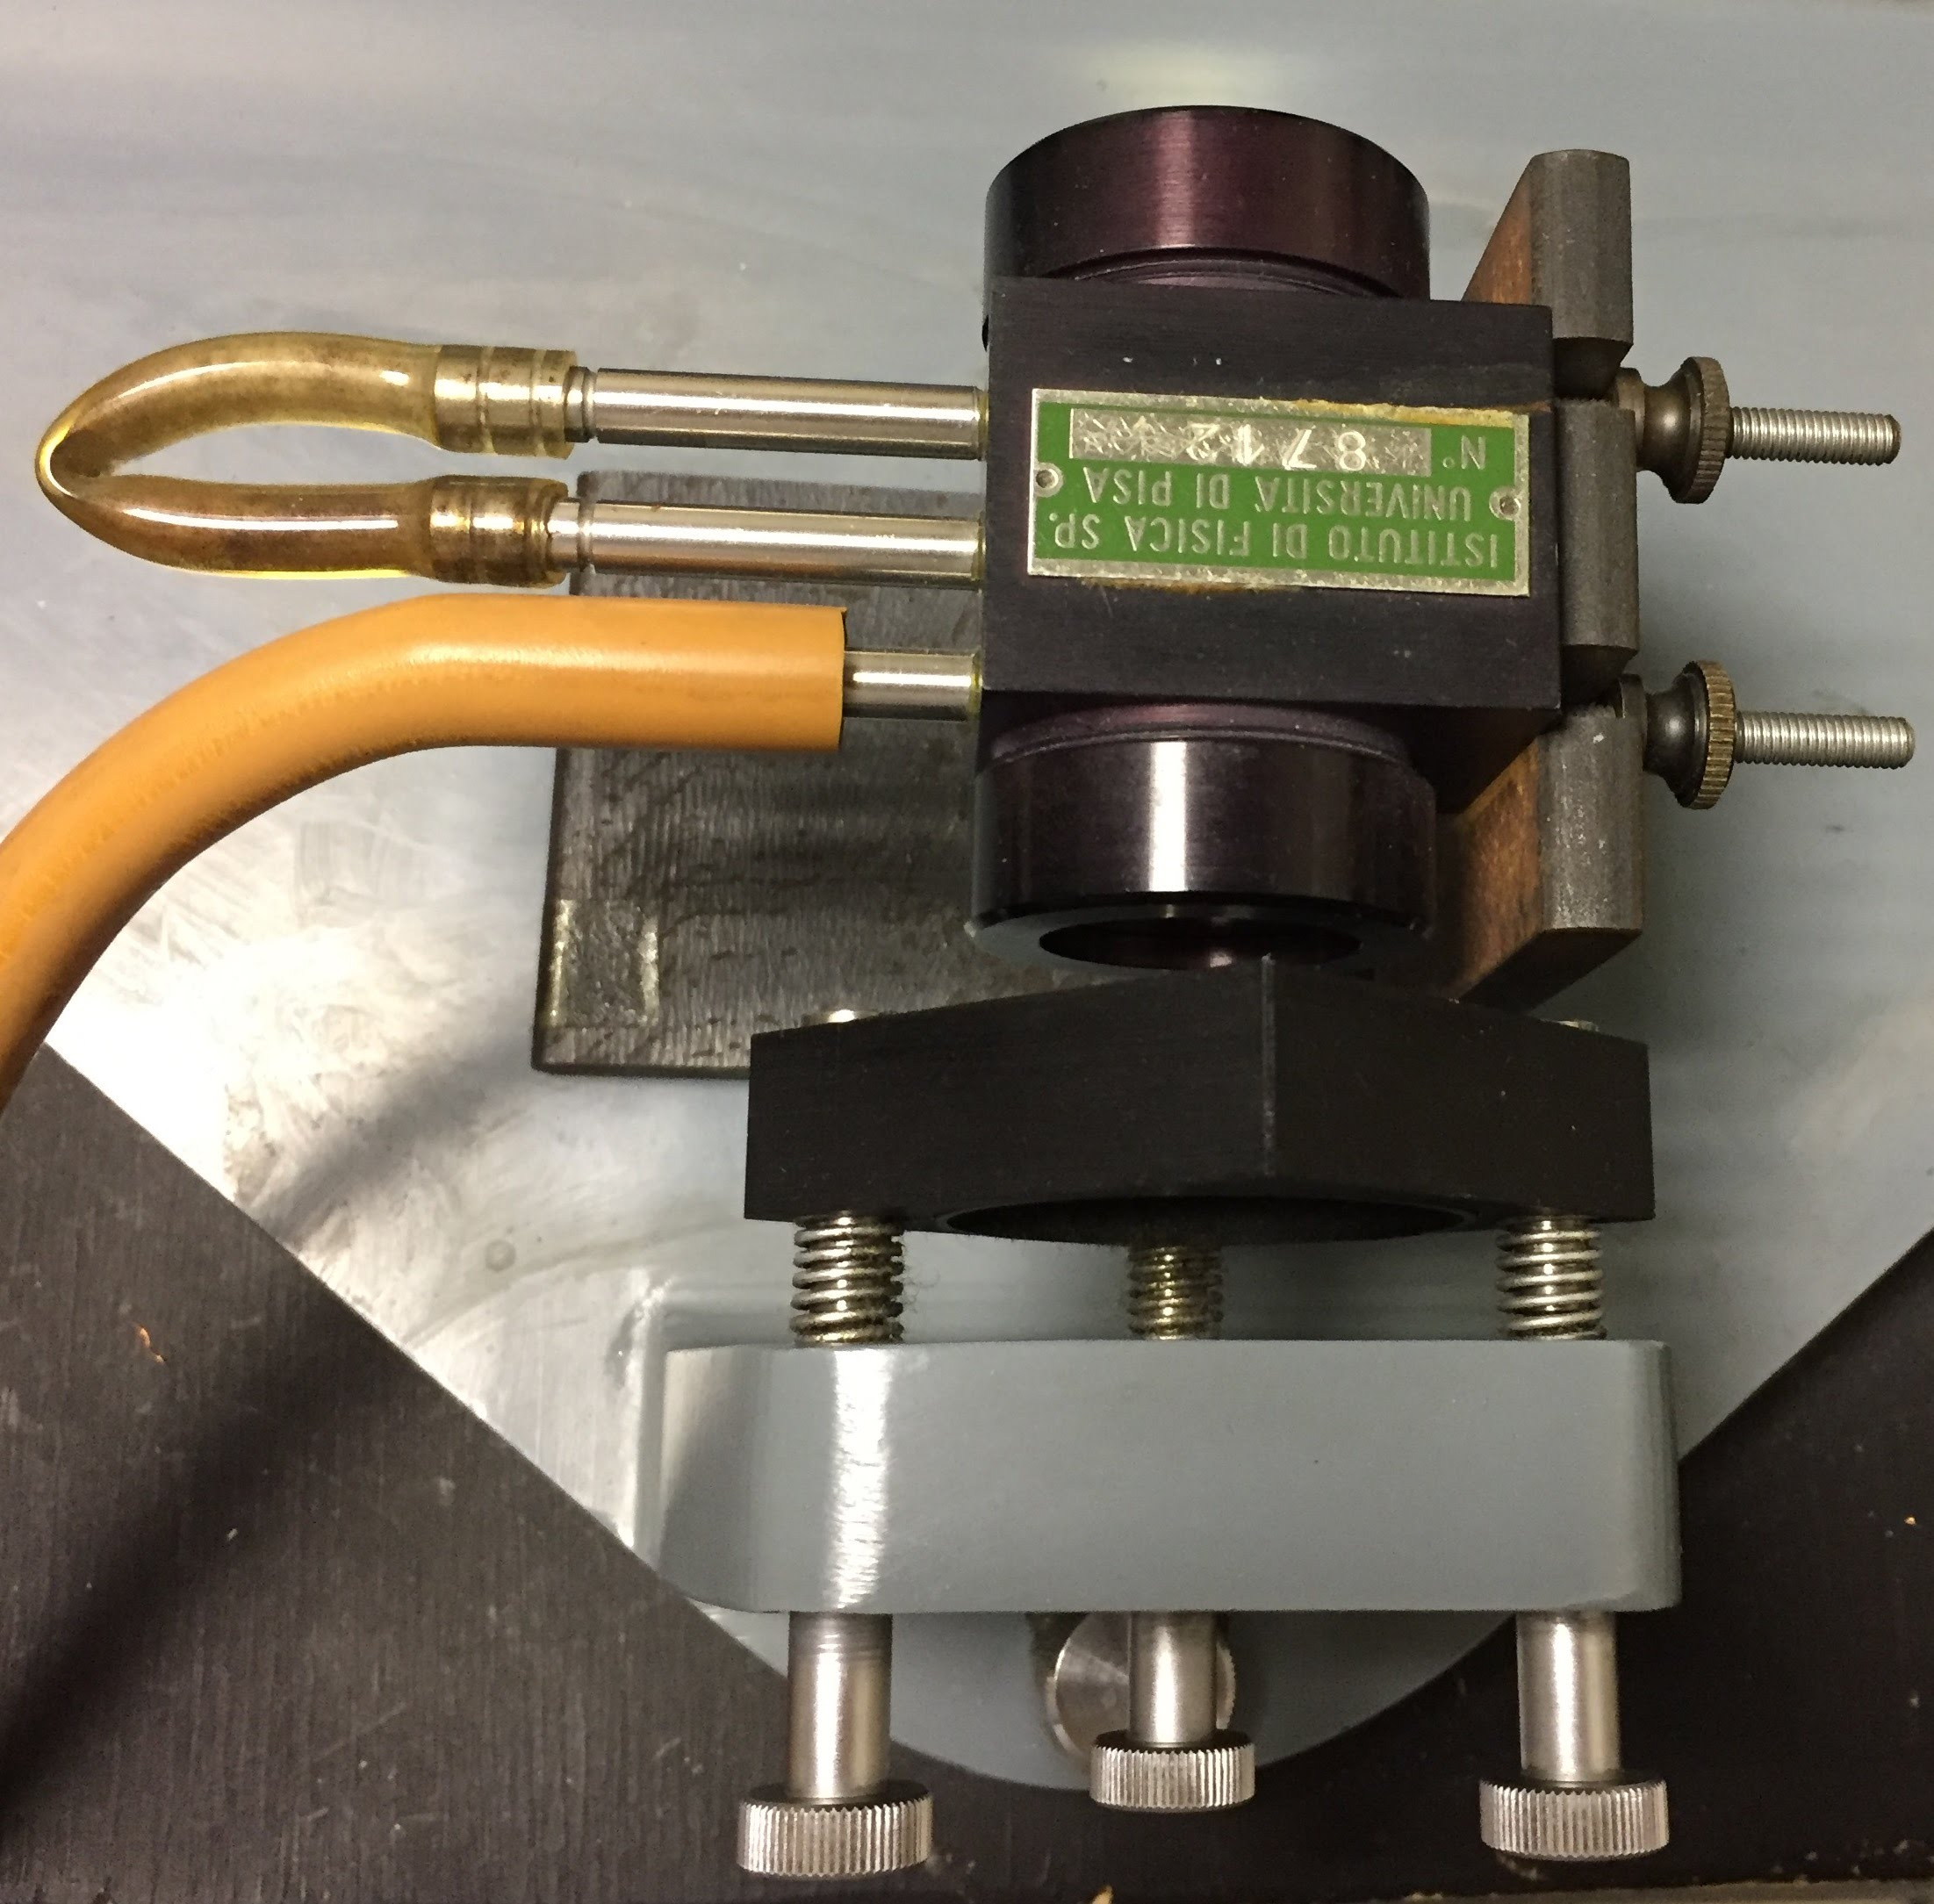
\includegraphics[width=0.3\textwidth]{cameravuoto.JPG}
 	\caption{Camera a vuoto.}
 	\label{fig:cv}
 \end{figure}

Dopodich� apriamo la camera cos� che si ristabilisca lentamente la pressione atmosferica al suo interno e contiamo il numero di frange dovute alla variazione dell'indice di rifrazione: il conteggio � stato effettuato osservando il numero di picchi presenti sul grafico mostratoci dal VI sullo schermo del PC. Abbiamo ripetuto le misure due volte per ognuno dei tre laser a nostra disposizione ottenendo entrambe le volte lo stesso numero di picchi; abbiamo quindi riportato tale valore una volta soltanto in Tabella \ref{tab:n}.

\subsection{Analisi dati}
Noto il numero di frange e nota la lunghezza d'onda del laser utilizzato � possibile ricavare la differenza $\Delta$n fra l'indice di rifrazione del vuoto (n=1) e quello dell'aria a pressione atmosferica e a temperatura ambiente tramite la relazione
\begin{equation}
\Delta n = \frac{m\lambda}{2d}
\end{equation}
dove d � la lunghezza della camera a vuoto.

Dal valore di $\Delta$n � quindi facile ricavare l'indice di rifrazione dell'aria presente nella stanza assumendo di essere riusciti a raggiungere all'interno della camera un vuoto tale da avere come condizione iniziale n=1. Abbiamo ottenuto i seguenti valori:

\begin{table}[H]
	\centering
	\begin{tabular}{|c|c|c|c|}
		\hline
		laser & $\lambda$ & frange  & $n(\Delta n)$ \\
		\hline
		HeNe & 632.8 & 43(1) &1.000272(6)\\
		rosso & 650 & 41(1) &1.000267(7)\\ 
		verde & 532 & 51(1) &1.000271(5)\\
		\hline
	\end{tabular}
	\caption{Indice di rifrazione dell'aria}
	\label{tab:n}
\end{table}

\subsection{Conclusioni}
Per poter effettuare un confronto con un modello teorico � necessario tenere presente la dipendenza dell'indice di rifrazione, oltre che dalla lunghezza d'onda della luce, dai parametri ambientali quali pressione, temperatura e umidit�. Il modello da noi considerato � la versione aggiornata da Birch e Downs dell'equazione di Edl�n.\footnote{ K.P. Birch and M.J. Downs, "An updated Edl�n equation for the refractive index of air," Metrologia 30, 155-162 (1993)}
Il calcolo dei valori teorici � stato effettuato attraverso un programma presente in rete al sito \texttt{http://emtoolbox.nist.gov/Wavelength/Documentation.asp}

Dato che non siamo a conoscenza dei valori di temperatura, pressione e umidit� all'interno del laboratorio abbiamo calcolato dei valori massimi e minimi dell'indice di rifrazione considerando degli intervalli dei parametri ambientali ragionevoli quali: $\Delta$T = 20-25 �C, $\Delta$P = 100-102 kPa e $\Delta$u = 30-70\%.\footnote{I valori della pressione sono stati scelti in base al grafico della pressione a Pisa nel mese di Novembre 2017 riportato nel sito \texttt{https://www.woitalia.it/weather/maps/city}}

\end{multicols}

\begin{table}[H]
	\centering
	\begin{tabular}{|c|c|c|c|c|}
		\hline
		laser & $\lambda$ & T=25�C, P=100 kPa, u=70\% & T=20�C, P=102 kPa, u=30\% & $n(\Delta n)$ \\
		\hline
		HeNe & 633 & 1.000263 & 1.000273 &1.000272(6)\\
		rosso & 650 & 1.000263 & 1.000273 &1.000267(7)\\ 
		verde & 532 & 1.000265 & 1.000275 &1.000271(5)\\
		\hline
	\end{tabular}
	\caption{Indice di rifrazione dell'aria}
	\label{tab:n}
\end{table}

\begin{multicols}{2}
Come si pu� vedere in tabella i valori misurati sono compatibili con gli intervalli ottenuti dal modello teorico considerato.

\end{multicols}

\end{document}
